\documentclass{protokol}
\leftheader{Mřížkový spektrometr}
\centerheader{Praktikum III}
\rightheader{Tomáš Derner}

\begin{document}

  \section*{Úkol}

    \begin{enumerate}
      \item Seřiďte spektrometr pro kolmý dopad světla pomocí bočního osvětlení nitkového kříže (rovina optické mřížky je kolmá k ose kolimátoru).
      \item Stanovte mřížkovou konstantu použité mřížky. K měření užijte čar sodíkového dubletu v 1. a 2. řádu.
      \item Odhadněte rozlišovací schopnost spektrometru ze zobrazení sodíkového dubletu ve spektru 1. a 2. řádu. Vypočtěte teoreticky maximální dosažitelnou rozlišovací schopnost a oba výsledky porovnejte.
      \item Proměřte viditelné čáry ve spektru rtuti v 1. řádu. S pomocí vámi stanovené mřížkové konstanty z úkolu 2. spočtěte vlnové délky rtuťového spektra a porovnejte je s tabelovanými hodnotami.
      \item Vytvořte kalibrační křivku spektrometru jako závislost vlnové délky na úhlu.
      \item Určete úhlovou disperzi mřížky ve žluté oblasti spektra 1. a 2. řádu. Vypočtěte teoretické hodnoty a porovnejte s experimentálními hodnotami.
      \item Spočtěte relativní chyby výsledků.
    \end{enumerate}

  \section*{Teorie}

    V tomto praktiku využijeme mřížkový spektrometr pro měření poloh spektrálních čar rtuťové výbojky. Použitá aparatura je popsaná v pokynech \cite{pokyny}.

    Pro získání mřížkové konstanty $a$ využijeme vzorec udávající úhlovou polohu $\varphi_k$ difrakčního maxima řádu $k$
    \begin{equation} \label{eq:a}
      \sin \varphi_k = \frac{k \lambda}{a},
    \end{equation}
    kde $\lambda$ je použitá vlnová délka.

    Protože poloha nultého maxima difrakčního vzoru nemusí nutně odpovídat nule na stupnici, měříme polohy spektrálních čar vždy na obou stranách a naměřené úhlové polohy $\psi_1$ a $\psi_2$ průměrujeme:
    \begin{equation}
      \varphi_k = \frac{|\psi_1 - \psi_2|}{2}.
    \end{equation}

    Rozlišovací schopnost mřížky je definovaná jako 
    \begin{equation}
      R = \frac{\lambda}{\delta \lambda},
    \end{equation}
    její teoretickou hodnotu lze spočítat podle vztahu
    \begin{equation} \label{eq:R_teorie}
      R_{teorie} = \num{0.82} \frac{D k}{a},
    \end{equation}
    kde $D = \SI{18}{mm}$ je průměr výstupní pupily kolimátoru \cite{pokyny}.

    Teoretickou úhlovou disperzi mřížkového spektrometru v určité oblasti spočteme podle vztahu
    \begin{equation} \label{eq:disperze_teorie}
      D_{a, teorie} = \frac{k}{a \cos \varphi},
    \end{equation}
    úhlovou disperzi z naměřených hodnot pak spočteme pomocí
    \begin{equation} \label{eq:disperze}
      D_a = \frac{\mathrm{d}\varphi}{\mathrm{d}\lambda},
    \end{equation}
    kde $\mathrm{d}\varphi$ je rozdíl poloh dvou blízkých proužků a $\mathrm{d}\lambda$ rozdíl odpovídajících vlnových délek.

  \section*{Výsledky}

    \subsection*{Úkol 2}

      Pomocí seřízeného mřížkového spektrometru byly naměřeny polohy sodíkového dubletu v nultém, prvním a druhém řádu na obou stranách. Výsledné hodnoty jsou zobrazeny na obrázku \ref{fig:sodik}. Chyba měření byla odhadnuta jako nejmenší možný rozdíl poloh, který lze odečíst ze stupnice (nikoli nejmenší rozdíl poloh, který je rozeznatelný dalekohledem).

      \begin{figure}[H]
        \centering
        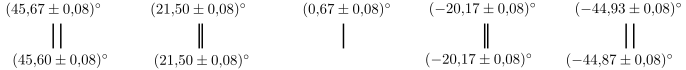
\includegraphics[width=\textwidth]{sodik}
        \caption{Naměřené hodnoty úhlových poloh proužků  sodíkového dubletu} 
        \label{fig:sodik}
      \end{figure}
 
      Pro určení mřížkové konstanty byly použity polohy sodíkového dubletu ve druhém maximu. Podle vzorce \eqref{eq:a} vychází pro $\lambda_1 \doteq \SI{589.00}{\nano\metre}$
      $$ a_1 = \SI{1.661 \pm 0.002}{\micro\metre}, $$
      pro $\lambda_2 \doteq \SI{589.59}{\nano\metre}$
      $$ a_2 = \SI{1.657 \pm 0.002}{\micro\metre}. $$

      Pro další výpočty budeme používat jejich průměrnou hodnotu
      $$ a = \SI{1.659 \pm 0.003}{\micro\metre}. $$
      Tato hodnota má relativní chybu $\SI{0.2}{\percent}$.

    \subsection*{Úkol 3}

      Je nutno oddělit schopnost opticky rozlišit jednotlivé spektrální čáry od schopnosti tyto rozdíly poloh odečíst na stupnici, tyto dvě hodnoty se totiž značně liší. Sodíkový dublet má mezi sebou mezeru $\approx \SI{0.6}{\nano\metre}$, v dalekohledu byly tyto dvě čáry jasně odděleny s velmi ostře definovanou tmavou oblastí mezi nimi. To přispělo k odhadu optické rozlišovací schopnosti v prvním řádu
      $$ \delta \lambda_{opt} = \SI{0.2}{\nano\metre}, $$
      $$ R_{opt} = \num{2945}. $$ 

      Na druhé straně stojí rozlišovací schopnost mřížkového spektrometru jakožto měřicího přístroje. Ta je kvůli nepříliš povedenému provedení stupnice tak nízká, že bylo možné odečíst rozdíl poloh čar sodíkového dubletu v prvním řádu. Rozlišovací schopnost spektrometru v prvním řádu byla proto odhadnuta na dvojnásobek této vzdálenosti,
      $$ \delta \lambda = \SI{1.2}{\nano\metre}, $$
      $$ R = \num{491}. $$

      Pomocí vztahu \eqref{eq:R_teorie} spočteme teoretickou rozlišovací schopnost 
      $$ R_{teorie} = \num{8897 \pm 16}. $$

    \subsection*{Úkol 4}

      V tabulce \ref{tab:rtut} jsou uvedeny naměřené hodnoty úhlových poloh spektrálních čar rtuťové výbojky společně s vypočítanými hodnotami vlnových délek a teoretických vlnových délek získaných z tabulky v praktiku. Chyba $\psi_1$ a $\psi_2$ byla odhadnuta jako výše.
      
      \begin{table}[H]
        \centering
        \setlength{\tabcolsep}{10pt}
        \begin{tabular}[t]{                                                                                           
  S[table-format=2.2]                                                                                         
  S[table-format=3.2]                                                                                         
  S[table-format=2.2]                                                                                         
  S[table-format=3.1]                                                                                         
  S[table-format=1.1]                                                                                         
  S[table-format=3.1]    
  r                                                                                     
} \toprule                                                                                                            
{$\psi_1$}         & {$\psi_2$}         & {$\varphi$}        & {$\lambda$}            & {$\sigma_\lambda$}     & {$\lambda_{teorie}$}   & barva       \\
{$[\si{\degree}]$} & {$[\si{\degree}]$} & {$[\si{\degree}]$} & {$[\si{\nano\metre}]$} & {$[\si{\nano\metre}]$} & {$[\si{\nano\metre}]$} &             \\ \midrule
14.65              & -13.52             & 14.08              & 403.7                  & 0.7                    & 404.7                  & fialová     \\
14.80              & -13.67             & 14.23              & 407.9                  & 0.7                    & 407.8                  & fialová     \\
15.75              & -14.63             & 15.19              & 434.7                  & 0.8                    & 433.9                  & modrá       \\
15.77              & -14.65             & 15.21              & 435.2                  & 0.8                    & 434.8                  & modrá       \\
15.78              & -14.67             & 15.23              & 435.7                  & 0.8                    & 435.8                  & modrá       \\
17.80              & -16.65             & 17.23              & 491.3                  & 0.9                    & 491.6                  & modrozelená \\
19.75              & -18.67             & 19.21              & 545.8                  & 1.0                    & 546.1                  & zelená      \\
20.88              & -19.80             & 20.34              & 576.7                  & 1.0                    & 577.0                  & žlutá       \\
21.00              & -19.87             & 20.43              & 579.2                  & 1.0                    & 579.1                  & žlutá       \\
22.01              & -20.98             & 21.50              & 608.0                  & 1.1                    & 607.3                  & červená     \\
22.23              & -21.15             & 21.69              & 613.2                  & 1.1                    & 612.3                  & červená     \\
22.63              & -21.58             & 22.11              & 624.4                  & 1.1                    & 623.4                  & červená     \\
24.37              & -23.35             & 23.86              & 671.0                  & 1.2                    & 671.6                  & červená     \\
25.08              & -24.13             & 24.61              & 690.8                  & 1.2                    & 690.7                  & červená     \\ \bottomrule
\end{tabular}                                                                                                      
                                                                                                              

        \caption{Naměřené a spočtené hodnoty pro zjištění poloh interferenčních proužků}
        \label{tab:rtut}
      \end{table}

    \subsection*{Úkol 5}

      Kalibrační křivka byla sestavena s pomocí hodnot z tabulky \ref{tab:rtut}. Hodnoty byly proloženy přímkou $\lambda = A \varphi + B$.
      
      $$ A = \SI{27.36 \pm 0.07}{}, $$
      $$ B = \SI{19 \pm 1}{}. $$

      \begin{figure}[H]
        \centering
        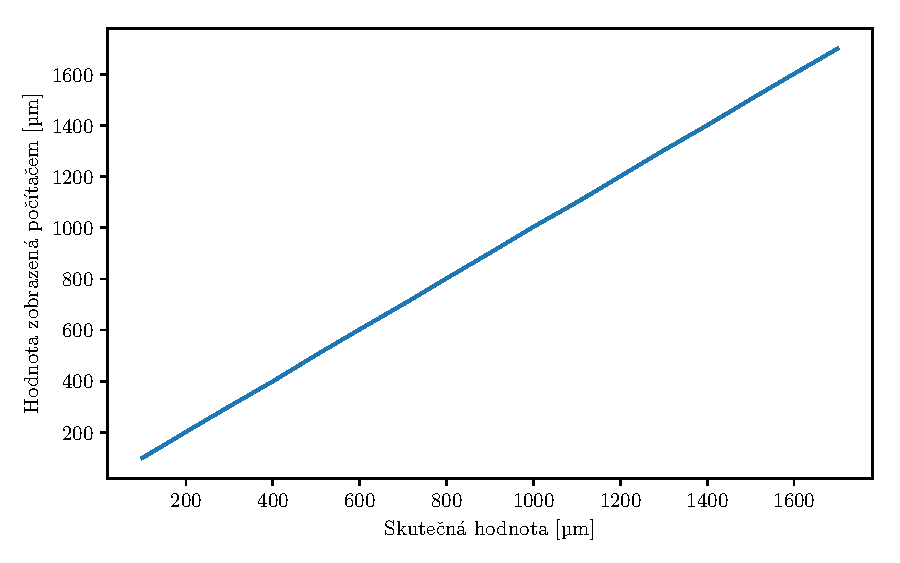
\includegraphics[]{kalibrace}
        \caption{Kalibrační křivka spektrometru}
        \label{fig:kalibrace}
      \end{figure}

    \subsection*{Úkol 6}

      Pomocí hodnot úhlů $\varphi$ žlutého dubletu rtuťové výbojky z tabulky \ref{tab:rtut} (přepočítaných na radiány) a vztahu \eqref{eq:disperze} spočteme úhlovou disperzi spektrometru v prvním řádu 
      $$ D_a = \SI{7 \pm 10 e5}{\per\metre}, $$
      protože však při výpočtu odečítáme velmi blízké hodnoty s nezanedbatelnou chybou, relativní chyba této veličiny převyšuje číslo 1 a činí tak tento výpočet zbytečným.
      Teoretickou hodnotu spočteme pro aritmetický průměr poloh dubletu podle \eqref{eq:disperze_teorie},
      $$ D_{a, teorie} = \SI{6.43 \pm 0.01 e5}{\per\metre}. $$ 
      Relativní chyba je $\SI{0.1}{\percent}$.

  \section*{Diskuse}

    Až na polohu prvního fialového proužku všechny interferenční proužky odpovídají v rámci chyby teoretickým hodnotám z tabulky v praktiku. Během měření byly pozorovány také spektrální čáry v oblasti modrozeleného a žlutého spektra, které v této tabulce nebyly uvedeny, nebyl na ně však brán zřetel.
  
    Jak již bylo řečeno výše, u této úlohy je významná skutečnost, že rozlišovací schopnost spektrometru jako takového se nemůže měřit s rozlišovací schopností optickou. Toto odrážejí zvolené hodnoty chyb. Z grafu \ref{fig:kalibrace} lze vyčíst, že kalibrační křivkou spektrometru je téměř dokonalá přímka, závislost úhlu na vlnové délce tedy není nijak deformovaná.

  \section*{Závěr}

    Spektrometr byl seřízen podle návodu.

    Z měření sodíkového dubletu byla získána mřížková konstanta 
    $$ a = \SI{1.659 \pm 0.003}{\micro\metre}. $$

    Byla odhadnuta rozlišovací schopnost spektrometru v prvním řádu 
    $$ R = \num{491}. $$

    Byly proměřeny spektrální čáry rtuťové výbojky. Z naměřených hodnot byly spočítány odpovídající vlnové délky. Následně byla vytvořena kalibrační křivka spektrometru.

    Byla spočtena teoretická hodnota úhlové disperze ve žluté oblasti spektra 
    $$ D_{a, teorie} = \SI{6.43 \pm 0.01 e5}{\per\metre}. $$
    Hodnota vypočtená z naměřených hodnot je bezvýznamná kvůli vysoké relativní chybě.

  \begin{thebibliography}{}
 
    \bibitem{pokyny}
    Pokyny k měření ``Mřížkový spektrometr'', dostupné z\\ \url{http://physics.mff.cuni.cz/vyuka/zfp/_media/zadani/pokyny/mereni_303.pdf}, 11.\,4.\,2018
   
  \end{thebibliography}

\end{document} 